
\section{Tema 1: Introducción y generalidades sobre metrología}
\subsection{Definiciones}
\begin{enumerate}
	\item \underline{\textbf{Magnitud}}: Atributo de un cuerpo que se puede distinguir cualitativamente y determinado cuantitativamente.
	\item \underline{\textbf{Magnitud básica}}: Magnitud que se acepta como independiente.
	\item \underline{\textbf{Magnitud derivada}}: Se define en a través de las magnitudes básicas.
	\item \underline{\textbf{Unidad de medida}}: Magnitud adoptada por convenio con la que se comparan magnitudes de la misma naturaleza.
	\item \underline{\textbf{Unidad coherente}}: Unidad derivada expresada como producto de potencias de unidades básicas.
	\item \underline{\textbf{Sistema de unidades}}: Conjunto de unidades básicas y derivadas. Cabe destacar el Sistema Internacional de Unidades que es un sistema coherente de unidades adaptado por la Conferencia General de Pesas y Medidas.
	\item \underline{\textbf{Valor de una magnitud}}: Expresión cuantitativa de una magnitud. Se expresa como una unidad de medida multiplicada por un número.
	\item \underline{\textbf{Valor verdadero}}: Valor que se obtendría a través de una medición perfecta de una magnitud. Este valor nunca se puede determinar, todas las medidas introducen incertidumbre.
	\item \underline{\textbf{Valor convencionalmente verdadero}}: Valor más probable que toma una magnitud. Se debe acompañar con su incertidumbre. Normalmente se corresponde con la media.
	\item \underline{\textbf{Medida}}: Conjunto de operaciones para determinar el valor de una magnitud. 
	\item \underline{\textbf{Medición general}}: Se determina el valor de una magnitud sobre la que se realiza alguna acción de control. Se realiza mediante aparatos convencionales.
	\item \underline{\textbf{Medición metrológica}}: Procedimiento plenamente especificado con el fin de calibrar o verificar un aparato. Se requieren aparatos patrones.
	\item \underline{\textbf{Mensurando}}: Magnitud sometida a medición.
	\item \underline{\textbf{Magnitud de influencia}}: Magnitudes que no son el objetivo de la medida pero alteran la medición.
	\item \underline{\textbf{Señal de medida}}: Magnitud que mantiene una relación funcional con el mensurando y lo representa.
	\item \underline{\textbf{Cadena de medida}}: Conjunto de instrumentos y personas que intervienen en una medición.
	\item \underline{\textbf{Valor nominal}}: Valor aproximado de una característica de un instrumento. 
	\item \underline{\textbf{Campo de medida (CM)}}: Valor máximo que puede indicar un aparato.
	\item \underline{\textbf{Rango de medida}}: Intervalo en el que el error debido al instrumento de medida se mantiene en unos límites especificados.
	\item \underline{\textbf{Constante de medida}}: Número por el que debe multiplicarse la medida de un instrumento para obtener el valor del mensurando. 
	\begin{center} 	Normalmente en un aparato analógico:\end{center}
		\[ k_m = \frac{CM}{Divisiones} \]
	\item \underline{\textbf{Estabilidad}}: Aptitud de un instrumento para mantener constantes sus características a lo largo del tiempo.
	\item \underline{\textbf{Transparencia}}: Aptitud de un instrumento para no alterar el mensurando.
	\item \underline{\textbf{Deriva}}: Variación lenta de una característica del instrumento por el paso del tiempo, mal uso o desgaste.
	\item \underline{\textbf{Zona muerta}}: Máxima variación de la señal de entrada sin que se perciba respuesta en la salida.
	\item \underline{\textbf{Sensibilidad}}: Variación de la salida ante un incremento de la entrada. No tienen porque ser siempre iguales.
	\[ S(x) = \frac{dx}{dy}=\frac{\bigtriangleup x}{\bigtriangleup y} \]
	\item \underline{\textbf{Resolución}}: Menor diferencia que puede apreciarse en un aparato de manera significativa.
	\begin{itemize}
	 \item En un aparato analógico suele tomarse como E/2 y como máximo E/4 donde E es una división de escala.
	 \item En un aparato digital se suele tomar su dígito menos significativo.
	\end{itemize}
	
	\begin{figure}[H]
		\centering
		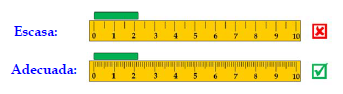
\includegraphics[width=0.5\textwidth]{imagenesTema1/resolucion.png}  
		\caption{Comparativa de resoluciones}
		\label{fig:sample}
	\end{figure}
	
	
	\item \underline{\textbf{Veracidad}}: Concordancia entre la media de un conjunto de medidas y un valor de referencia. Normalmente se comprueba si un valor nominal es correcto.
	\item \underline{\textbf{Precisión}}: Capacidad de un instrumento para dar valores agrupados al repetir medidas.
	\item \underline{\textbf{Exactitud}}: Grado de concordancia entre un valor medido y el verdadero. Requiere veracidad y precisión.
	\item \underline{\textbf{Sesgo}}: Diferencia entre la media de las medidas y el valor de referencia.
	\item \underline{\textbf{Linealidad}}: Indica la evolución del sesgo a lo largo del campo de medida del aparato.
	
	\begin{figure}[H]
		\centering
		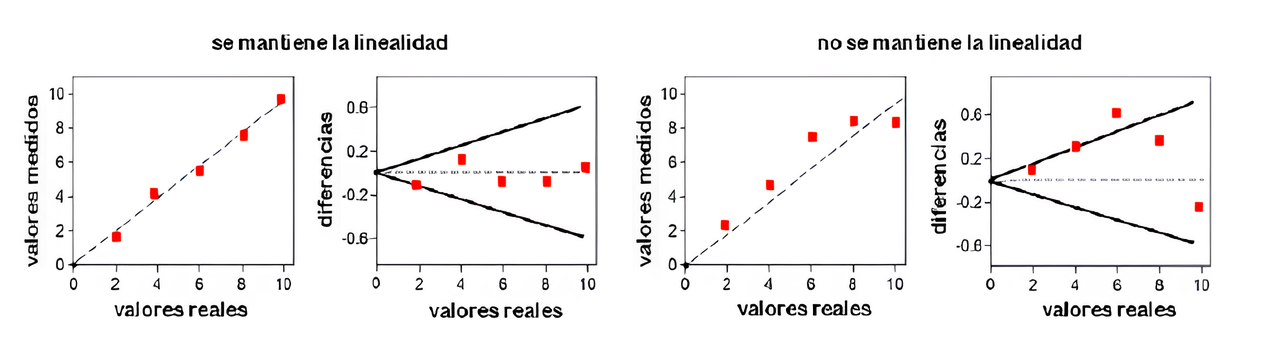
\includegraphics[width=1\textwidth]{imagenesTema1/linealidad.png}  
		\caption{Comparativa de resoluciones}
		\label{fig:sample}
	\end{figure}
	
	\item \underline{\textbf{Índice de clase}}:
	\item \underline{\textbf{Incertidumbre de medida}}:
	\item \underline{\textbf{Error de medida }}:
	\item \underline{\textbf{Error aleatorio}}:
	\item \underline{\textbf{Error sistemático}}:
	\item \underline{\textbf{Tolerancia}}:
	\item \underline{\textbf{Incertidumbre}}:
\end{enumerate}
\subsection{Causas de errores}
\subsection{Ley propagación de incertidumbres}
\subsection{Estimación de la incertidumbre}
\subsection{Relación tolerancia incertidumbre}
\subsection{Relación incertidumbre resolución}

